\documentclass[9pt]{beamer}
\usetheme{Antibes}
\useinnertheme{rectangles}
\useoutertheme{infolines}
\usepackage[utf8]{inputenc}
\usepackage[T1]{fontenc}
\usepackage[ngerman]{babel}

% Patch the look of +, = in arev
\usefonttheme{serif} 

\usepackage{arev}
\usepackage{amsmath}
\usepackage{amssymb}

% Patch punctuation to be upright
\DeclareMathSymbol{.}{\mathpunct}{operators}{`.}
\DeclareMathSymbol{,}{\mathpunct}{operators}{`,}

\setbeamertemplate{footline}{%
\begin{beamercolorbox}[ht=3.0ex,dp=1ex]{title in head/foot}
\hfill\footnotesize\insertpagenumber\enspace\enspace\end{beamercolorbox}}

\definecolor{bluegreen1}{rgb}{0.0,0.20,0.28}
\definecolor{bluegreen2}{rgb}{0.0,0.20,0.28}
\setbeamercolor*{palette primary}{fg=white,bg=bluegreen1}
\setbeamercolor*{palette secondary}{fg=white,bg=bluegreen2}
\setbeamercolor*{palette tertiary}{fg=white,bg=bluegreen2}
\setbeamercolor{itemize item}{fg=black}
\setbeamercolor{block title}{bg=bluegreen2}
\newcommand{\modest}[1]{{\small\color{gray}#1}}

\newcommand{\ee}{\mathrm e}
\newcommand{\ui}{\mathrm i}
\newcommand{\real}{\operatorname{Re}}
\newcommand{\imag}{\operatorname{Im}}
\newcommand{\uv}[1]{\underline{#1}}
\newcommand{\bv}[1]{\mathbf{#1}}

\newcommand{\N}{\mathbb N}
\newcommand{\Z}{\mathbb Z}
\newcommand{\Q}{\mathbb Q}
\newcommand{\R}{\mathbb R}
\newcommand{\C}{\mathbb C}

\newcommand{\id}{\operatorname{id}}
\newcommand{\sgn}{\operatorname{sgn}}
\newcommand{\Abb}{\operatorname{Abb}}
\newcommand{\unit}[1]{\mathrm{#1}}
\newcommand{\chem}[1]{\mathrm{#1}}
\newcommand{\strong}[1]{\textsf{\textbf{#1}}}
\newcommand{\defiff}{\quad:\Longleftrightarrow\quad}
\renewcommand{\qedsymbol}{\ensuremath{\Box}}

\newcommand{\icol}[1]{
  \big(\!\begin{smallmatrix}#1\end{smallmatrix}\!\big)%
}

\newcommand{\parspace}{\vspace{0.8em}}


\title{Was ist ein Vektor?}
\date{}

\begin{document}

\begin{frame}
\maketitle
\end{frame}

\begin{frame}
Betrachten wir eine Ebene, darin einen beliebigen Punkt $P$. Ein
Vektor $\bv v$ stellt eine Verschiebung von $P$ zu einem Punkt $P'$
dar.\pause

\vspace{-1em}
\begin{center}
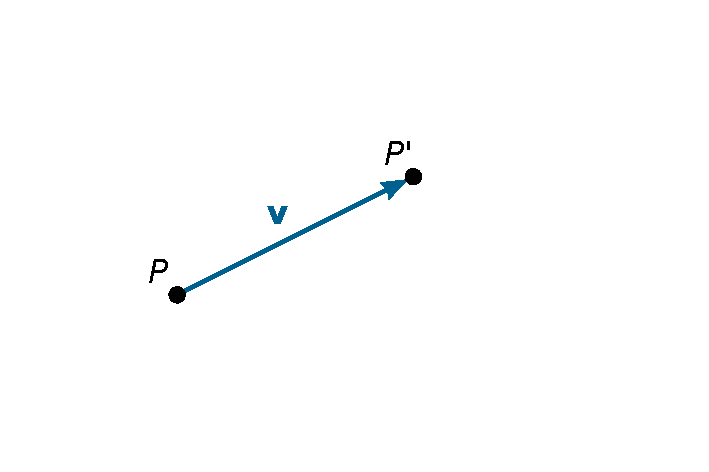
\includegraphics[width=64mm]{img/vec-p-pprime.pdf}
\end{center}
\end{frame}

\begin{frame}[t]
\vspace{1em}
Die Einführung eines Koordinatensystems erlaubt die Darstellung der
Punkte durch Koordinaten.

\parspace
Wir schreiben $P=\icol{x\\ y}$ und
$P'=\icol{x'\\ y'}$. Sei z.\,B. $P:=\icol{2\\ 2}$ und $P':=\icol{6\\ 4}$.\pause

\parspace
Dies führt zur Darstellung von $\bv v$ als die Verschiebung von
Koordinaten, d.\,h. $x' = x+v_1$ und $y' = y+v_2$.\pause

\vspace{-1em}
\begin{center}
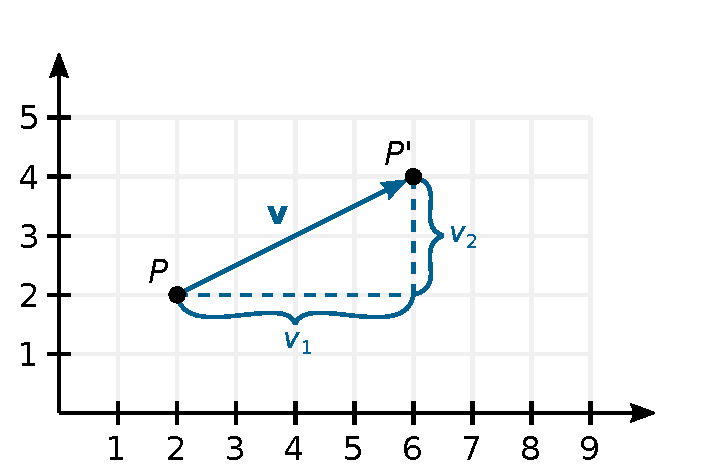
\includegraphics[width=64mm]{img/vec-p-pprime-coord.pdf}
\end{center}
\end{frame}

\begin{frame}
Man definiert nun
\[\bv v := \begin{pmatrix}v_1\\ v_2\end{pmatrix},\qquad
\begin{pmatrix}x\\ y\end{pmatrix} + \begin{pmatrix}v_1\\ v_2\end{pmatrix}
:= \begin{pmatrix}x+v_1\\ y+v_2\end{pmatrix},\]
denn die Verschiebung ist dann beschrieben durch
\[P' = P + \bv v.\]\pause
Mit
\[\begin{pmatrix}x'\\ y'\end{pmatrix} - \begin{pmatrix}x\\ y\end{pmatrix}
:= \begin{pmatrix}x'-x\\ y'-y\end{pmatrix}\]
gilt entsprechend
\[\bv v = P' - P.\]
\end{frame}

\begin{frame}
\begin{center}
\strong{Addition von Vektoren}
\end{center}
\end{frame}

\begin{frame}
Die Addition von Vektoren ist definiert als die Hintereinanderausführung
der Verschiebungen.

\parspace
Das heißt, ist $P' = P+\bv v$ und $P'' = P'+\bv w$,
dann ist $P'' = P+(\bv v+\bv w)$.\pause

\parspace
Es gilt
\[\begin{pmatrix}v_1\\ v_2\end{pmatrix} + \begin{pmatrix}w_1\\ w_2\end{pmatrix}
= \begin{pmatrix}v_1+w_1\\ v_2+w_2\end{pmatrix}.\]\pause
\strong{Beweis.} Einsetzen ergibt
\[\bv v+\bv w = P''-P = (P'+\bv w)-P = ((P+\bv v)+\bv w)-P.\]
Die Operationen auf der rechten Seite wurden definiert. Das macht
\[\begin{pmatrix}v_1\\ v_2\end{pmatrix} + \begin{pmatrix}w_1\\ w_2\end{pmatrix}
= \begin{pmatrix}x + v_1 + w_1 - x\\ y + v_2 + w_2 - y\end{pmatrix}
= \begin{pmatrix}v_1 + w_1\\ v_2 + w_2\end{pmatrix}.\;\qedsymbol\]
\end{frame}

\begin{frame}
\strong{Beispiel.} Sei
\[P:=\icol{2\\ 1},\quad
\bv v := \icol{4\\ 1},\quad \bv w := \icol{1\\ 2}.\]\pause
Das macht
\[P' = \icol{6\\ 2},\quad P'' = \icol{7\\ 4}, \quad\bv v+\bv w = \icol{5\\ 3}.\]

\vspace{-1em}
\begin{center}
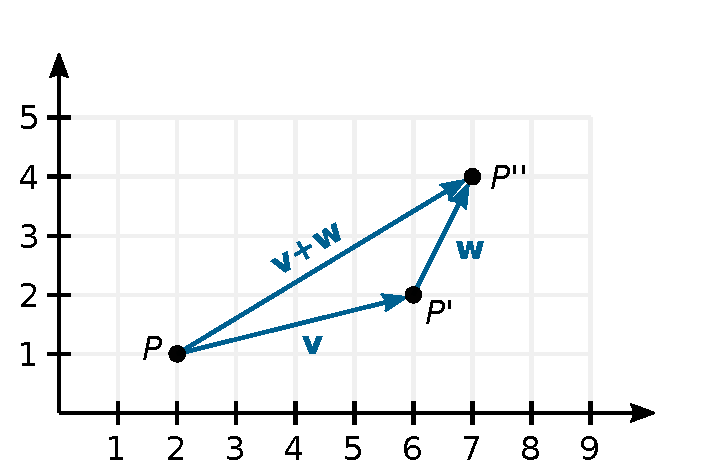
\includegraphics[width=64mm]{img/vec-addition.pdf}
\end{center}
\end{frame}

\begin{frame}
\begin{center}
\strong{Ortsvektoren}
\end{center}
\end{frame}

\begin{frame}
Wir beobachten, dass man
\[\begin{pmatrix}x\\ y\end{pmatrix}
= \begin{pmatrix}0\\ 0\end{pmatrix} + \begin{pmatrix}x\\ y\end{pmatrix}\]
rechnen kann. Das bedeutet, jedem Punkt in der Ebene entspricht genau
ein Vektor mit den gleichen Koordinaten, der vom Ursprung auf den Punkt
verschiebt.\pause

\parspace
Einen solchen an den Ursprung angehefteten Vektor nennen wir \emph{Ortsvektor}.\pause

\parspace
Im Gegensatz zu einem gewöhnlichen Vektor verändert sich ein Ortsvektor
bei Translation (Parallelverschiebung) des Koordinatensystems.
\end{frame}

\begin{frame}
\begin{center}
\strong{Skalarmultiplikation}
\end{center}
\end{frame}

\begin{frame}
Für eine reelle Zahl $r$ definiert man
\[r\cdot\begin{pmatrix}v_1\\ v_2\end{pmatrix}
= \begin{pmatrix}r\cdot v_1\\ r\cdot v_2\end{pmatrix}.\]\pause
Dies dient zur Skalierung von Vektoren. Z.\,B. gilt
\begin{gather*}
2\bv v = \bv v + \bv v,\\
\tfrac{1}{2}\bv v + \tfrac{1}{2}\bv v = \bv v.
\end{gather*}
Demzufolge ist $2\bv v$ die doppelte und $\tfrac{1}{2}\bv v$ die halbe
Verschiebung.
\end{frame}

\begin{frame}
\begin{center}
\strong{Standardbasis}
\end{center}
\end{frame}

\begin{frame}
Mit den Operationen und Addition und Skalarmultiplikation kann man
jeden Vektor $\bv v$ zerlegen in
\[\bv v = \begin{pmatrix}v_1\\ v_2\end{pmatrix}
= \begin{pmatrix}v_1\\ 0\end{pmatrix}
+ \begin{pmatrix}0\\ v_2\end{pmatrix}
= v_1\begin{pmatrix}1\\ 0\end{pmatrix}
+ v_2\begin{pmatrix}0\\ 1\end{pmatrix}.\]\pause
Die beiden Vektoren
\[\bv e_1 = \begin{pmatrix}1\\ 0\end{pmatrix},\quad
\bv e_2 = \begin{pmatrix}0\\ 1\end{pmatrix}\]
nennen wir \emph{Basisvektoren}. Sie bilden die \emph{Standardbasis}
des Koordinatenraums $\R^2$.
\end{frame}

\begin{frame}
\strong{Bemerkung.}
Allgemein nennt man zwei Vektoren $\bv a_1,\bv a_2$ eine Basis,
wenn sich jeder Vektor $\bv v$ in der Form
\[\bv v = \lambda_1\bv a_1 + \lambda_2\bv a_2\]
darstellen lässt. Die rechte Seite der Gleichung wird
\emph{Linearkombination} von $\bv a_1$ und $\bv a_2$ genannt.
\end{frame}

\begin{frame}
\begin{center}
\strong{Betrag}
\end{center}
\end{frame}

\begin{frame}
Der Betrag $|\bv v|$ eines Vektors $\bv v = \icol{v_1\\ v_2}$ ist seine Länge.\pause

\parspace
Zur Berechnung ziehen wir den Satz des Pythagoras heran und erhalten
\[|\bv v|^2 = v_1^2+v_2^2.\]\pause
Es gilt die Rechenregel
\[|r\cdot\bv v| = |r|\cdot|\bv v|,\]
denn
\[|r\cdot\bv v|^2 = |\icol{rv_1\\ rv_2}|^2
= (rv_1)^2+(rv_2)^2 = r^2(v_1^2+v_2^2) = r^2\cdot |\bv v|^2.\]
\end{frame}

\begin{frame}
Ende.
\vfill\hfill\modest{Juli 2020}\\
\hfill\modest{Creative Commons CC0 1.0}
\end{frame}


\end{document}


